\documentclass[tikz,border=2pt]{standalone}

\usepackage{tikz}
\usetikzlibrary{positioning,arrows.meta,fit,calc,backgrounds}

\definecolor{slate900}{HTML}{0F172A}
\definecolor{slate700}{HTML}{334155}
\definecolor{slate500}{HTML}{64748B}
\definecolor{slate300}{HTML}{CBD5E1}
\definecolor{slate200}{HTML}{E2E8F0}
\definecolor{slate100}{HTML}{F1F5F9}
\definecolor{blue700}{HTML}{2563EB}
\definecolor{blue100}{HTML}{DBEAFE}
\definecolor{teal700}{HTML}{0F766E}
\definecolor{teal100}{HTML}{CCFBF1}
\definecolor{amber700}{HTML}{D97706}
\definecolor{amber100}{HTML}{FEF3C7}

\begin{document}
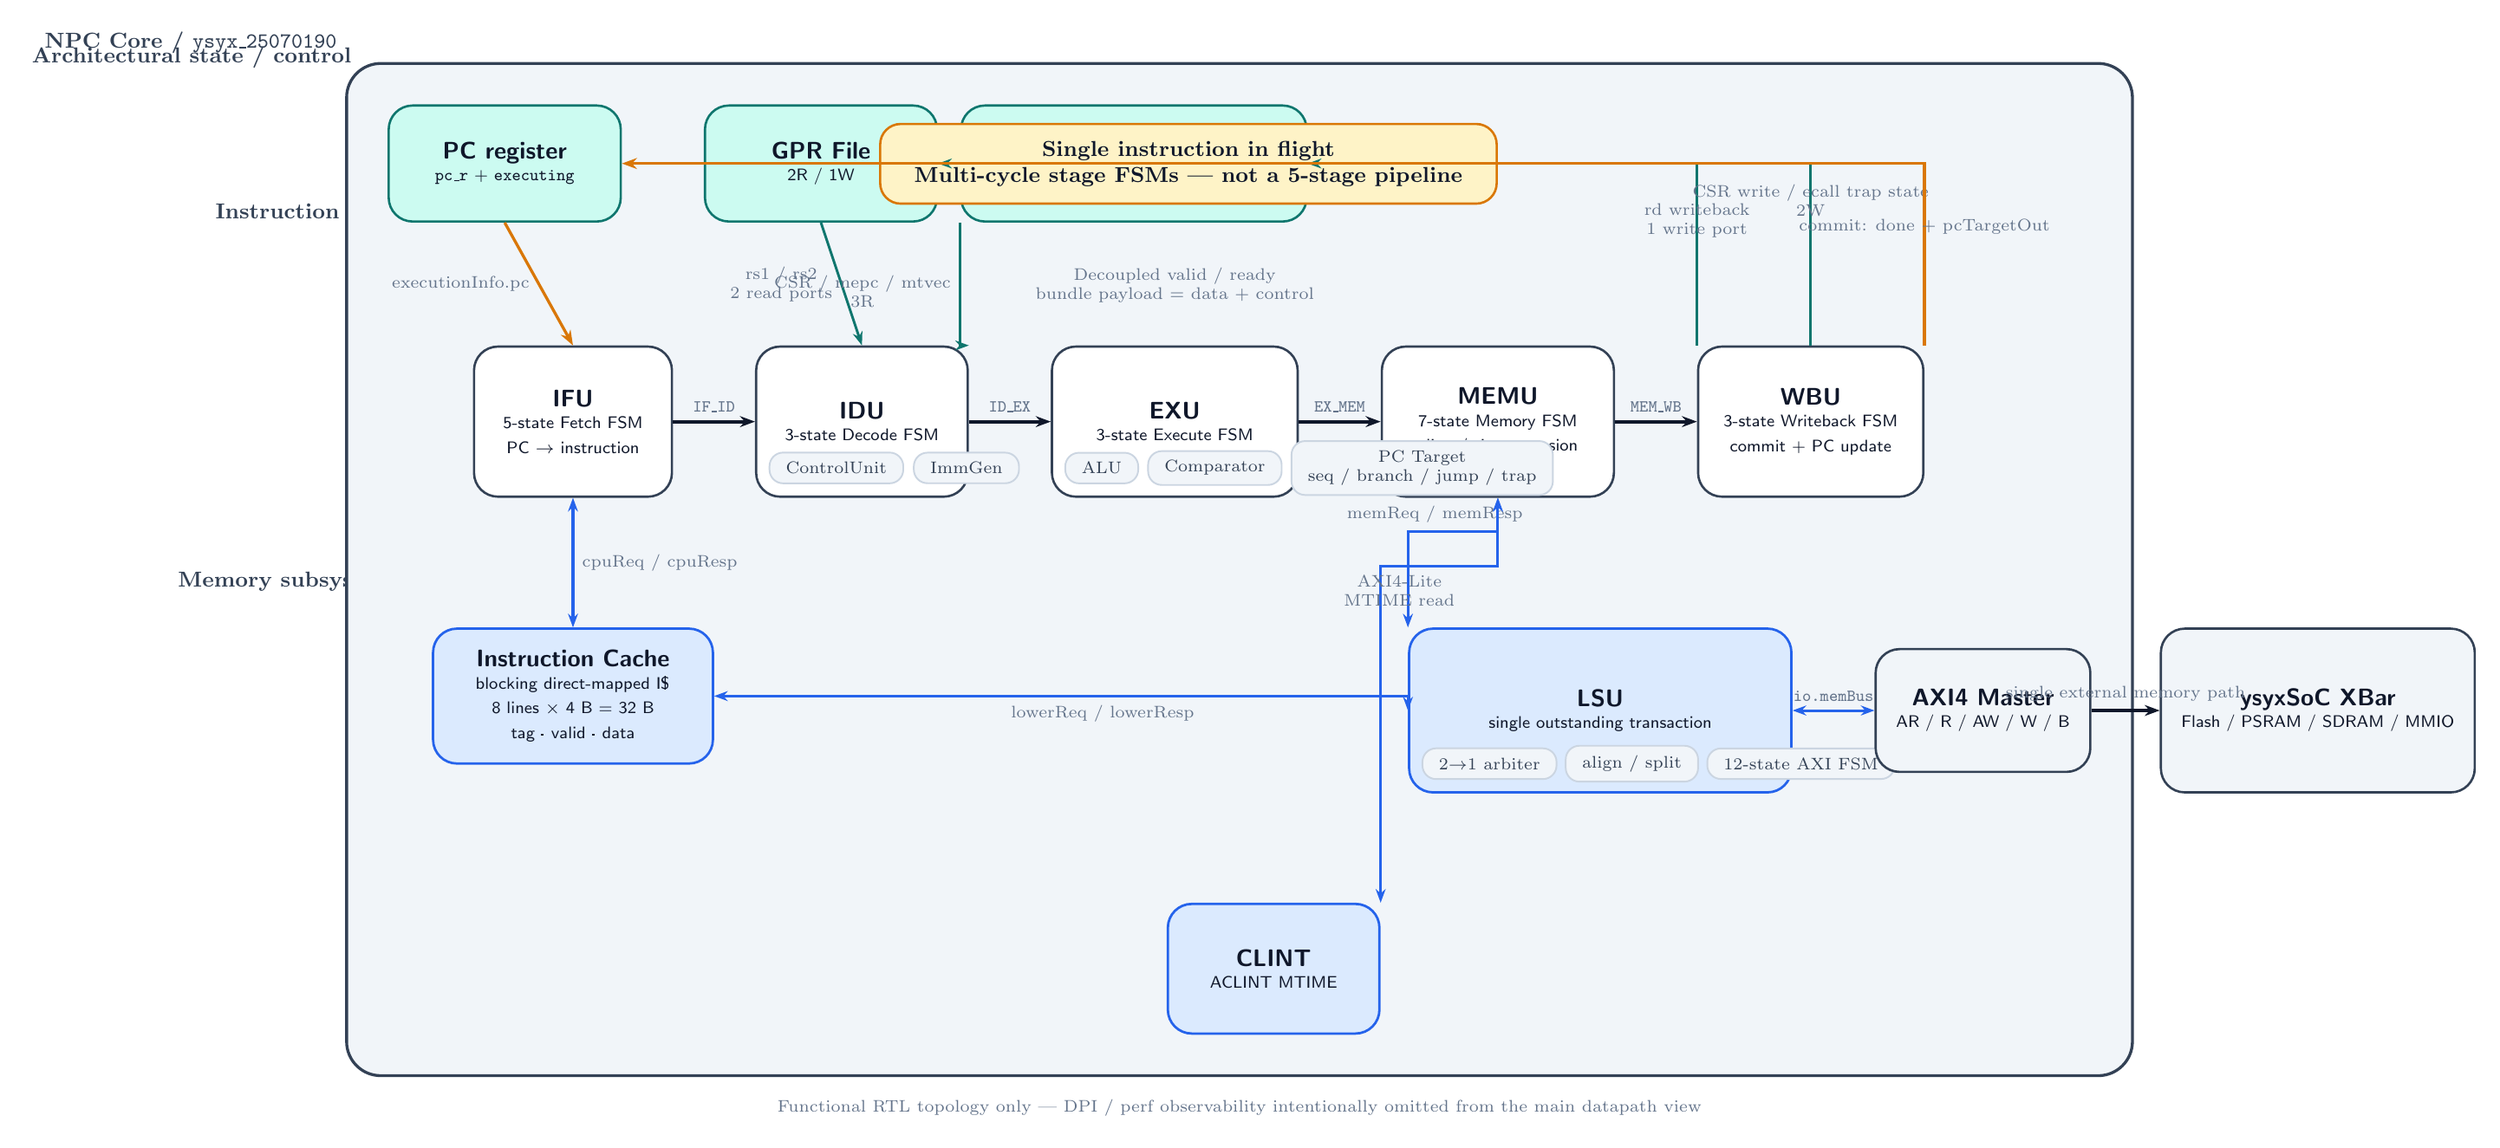
\begin{tikzpicture}[
  font=\sffamily,
  node distance=8mm and 10mm,
  stage/.style={
    draw=slate700,
    rounded corners=3.5mm,
    fill=white,
    line width=0.95pt,
    minimum height=22mm,
    minimum width=27mm,
    align=center,
    text=slate900,
    inner sep=3.2mm
  },
  stagewide/.style={stage, minimum width=36mm},
  statebox/.style={
    draw=teal700,
    rounded corners=3.5mm,
    fill=teal100,
    line width=0.95pt,
    minimum height=17mm,
    minimum width=30mm,
    align=center,
    inner sep=3mm,
    text=slate900
  },
  memorybox/.style={
    draw=blue700,
    rounded corners=3.5mm,
    fill=blue100,
    line width=1pt,
    minimum height=19mm,
    minimum width=36mm,
    align=center,
    inner sep=3.2mm,
    text=slate900
  },
  externalbox/.style={
    draw=slate700,
    rounded corners=3.5mm,
    fill=slate100,
    line width=0.95pt,
    minimum height=18mm,
    minimum width=32mm,
    align=center,
    inner sep=3mm,
    text=slate900
  },
  subunit/.style={
    draw=slate300,
    rounded corners=2mm,
    fill=slate100,
    line width=0.7pt,
    inner xsep=2.4mm,
    inner ysep=1.4mm,
    font=\scriptsize,
    text=slate700,
    align=center
  },
  stageflow/.style={draw=slate900, line width=1.35pt, -{Stealth[length=2.2mm,width=1.6mm]}},
  memflow/.style={draw=blue700, line width=1.1pt, {Stealth[length=2mm,width=1.45mm]}-{Stealth[length=2mm,width=1.45mm]}},
  regflow/.style={draw=teal700, line width=1.05pt, -{Stealth[length=2mm,width=1.45mm]}},
  controlflow/.style={draw=amber700, line width=1.2pt, -{Stealth[length=2.2mm,width=1.6mm]}},
  tap/.style={draw=slate500, dashed, line width=0.8pt},
  annotation/.style={font=\scriptsize, text=slate500, align=center},
  sectionbox/.style={
    draw=none,
    rounded corners=4mm,
    fill=slate100,
    inner sep=4mm
  },
  sectionlabel/.style={font=\bfseries\small, text=slate700},
  boundary/.style={
    draw=slate700,
    rounded corners=5mm,
    fill=slate100,
    line width=1.2pt,
    inner sep=6mm
  },
  banner/.style={
    draw=amber700,
    rounded corners=3mm,
    fill=amber100,
    line width=0.95pt,
    inner xsep=5mm,
    inner ysep=2.5mm,
    align=center,
    text=slate900,
    font=\bfseries\small
  }
]

% Central lifecycle
\node[stage, minimum width=29mm] (ifu) {
  {\bfseries IFU}\\[-1mm]
  {\scriptsize 5-state Fetch FSM}\\[-0.6mm]
  {\scriptsize PC $\rightarrow$ instruction}
};
\node[stage, minimum width=31mm, right=12mm of ifu] (idu) {
  {\bfseries IDU}\\[-1mm]
  {\scriptsize 3-state Decode FSM}
};
\node[stagewide, right=12mm of idu] (exu) {
  {\bfseries EXU}\\[-1mm]
  {\scriptsize 3-state Execute FSM}
};
\node[stage, minimum width=34mm, right=12mm of exu] (memu) {
  {\bfseries MEMU}\\[-1mm]
  {\scriptsize 7-state Memory FSM}\\[-0.6mm]
  {\scriptsize align / sign extension}
};
\node[stage, minimum width=33mm, right=12mm of memu] (wbu) {
  {\bfseries WBU}\\[-1mm]
  {\scriptsize 3-state Writeback FSM}\\[-0.6mm]
  {\scriptsize commit + PC update}
};

\draw[stageflow] (ifu.east) -- node[above, annotation] {\texttt{IF\_ID}} (idu.west);
\draw[stageflow] (idu.east) -- node[above, annotation] {\texttt{ID\_EX}} (exu.west);
\draw[stageflow] (exu.east) -- node[above, annotation] {\texttt{EX\_MEM}} (memu.west);
\draw[stageflow] (memu.east) -- node[above, annotation] {\texttt{MEM\_WB}} (wbu.west);
\node[annotation, above=5mm of exu] (bundle-note) {Decoupled valid / ready\\bundle payload = data + control};

% Stage internals
\node[subunit, anchor=south west] (idu-cu) at ($(idu.south west)+(2mm,2mm)$) {ControlUnit};
\node[subunit, right=1.3mm of idu-cu] (idu-imm) {ImmGen};

\node[subunit, anchor=south west] (exu-alu) at ($(exu.south west)+(2mm,2mm)$) {ALU};
\node[subunit, right=1.2mm of exu-alu] (exu-comp) {Comparator};
\node[subunit, right=1.2mm of exu-comp] (exu-pc) {PC Target\\seq / branch / jump / trap};

% Architectural state
\node[statebox, above=18mm of ifu, xshift=-10mm, minimum width=34mm] (pcstate) {
  {\bfseries PC register}\\[-1mm]
  {\scriptsize \texttt{pc\_r} + \texttt{executing}}
};

\node[statebox, above=18mm of idu, xshift=-6mm, minimum width=34mm] (gpr) {
  {\bfseries GPR File}\\[-1mm]
  {\scriptsize 2R / 1W}
};

\node[statebox, above=18mm of exu, xshift=-6mm, minimum width=42mm] (csr) {
  {\bfseries CSR File}\\[-1mm]
  {\scriptsize 3R / 2W}\\[-0.6mm]
  {\scriptsize mstatus \textperiodcentered{} mtvec \textperiodcentered{} mepc \textperiodcentered{} mcause \textperiodcentered{} mtval}
};

\node[banner, above=8mm of bundle-note, xshift=2mm] (banner) {Single instruction in flight\\Multi-cycle stage FSMs --- not a 5-stage pipeline};

% Memory subsystem
\node[memorybox, below=19mm of ifu, minimum width=41mm] (icache) {
  {\bfseries Instruction Cache}\\[-1mm]
  {\scriptsize blocking direct-mapped I\$}\\[-0.6mm]
  {\scriptsize 8 lines $\times$ 4 B = 32 B}\\[-0.6mm]
  {\scriptsize tag \textperiodcentered{} valid \textperiodcentered{} data}
};

\node[memorybox, below=19mm of memu, xshift=15mm, minimum width=56mm, minimum height=24mm] (lsu) {
  {\bfseries LSU}\\[-1mm]
  {\scriptsize single outstanding transaction}
};
\node[subunit, anchor=south west] (lsu-arb) at ($(lsu.south west)+(2mm,2mm)$) {2$\rightarrow$1 arbiter};
\node[subunit, right=1.1mm of lsu-arb] (lsu-align) {align / split};
\node[subunit, right=1.1mm of lsu-align] (lsu-fsm) {12-state AXI FSM};

\node[memorybox, below left=16mm and 4mm of lsu, minimum width=31mm] (clint) {
  {\bfseries CLINT}\\[-1mm]
  {\scriptsize ACLINT MTIME}
};

\node[externalbox, right=12mm of lsu, minimum width=30mm] (axi) {
  {\bfseries AXI4 Master}\\[-1mm]
  {\scriptsize AR / R / AW / W / B}
};

\node[externalbox, right=10mm of axi, minimum width=37mm, minimum height=24mm] (soc) {
  {\bfseries ysyxSoC XBar}\\[-1mm]
  {\scriptsize Flash / PSRAM / SDRAM / MMIO}
};

% Primary connections
\draw[controlflow] (pcstate.south) -- node[left, annotation] {executionInfo.pc} (ifu.north);
\draw[memflow] (ifu.south) -- node[right, annotation] {cpuReq / cpuResp} (icache.north);
\draw[memflow] (icache.east) -| node[pos=0.28, below, annotation] {lowerReq / lowerResp} (lsu.west);
\draw[memflow] (memu.south) -- ++(0,-5mm) -| node[pos=0.35, above, annotation] {memReq / memResp} (lsu.north west);
\draw[memflow] (memu.south) -- ++(0,-10mm) -| node[pos=0.42, below, annotation] {AXI4-Lite\\MTIME read} (clint.north east);
\draw[memflow] (lsu.east) -- node[above, annotation] {\texttt{io.memBus}} (axi.west);
\draw[stageflow] (axi.east) -- node[above, annotation] {single external memory path} (soc.west);

% Register file / CSR paths
\draw[regflow] (gpr.south) -- node[left, annotation] {rs1 / rs2\\2 read ports} (idu.north);
\draw[regflow] (csr.south west) |- node[pos=0.28, left, annotation] {CSR / mepc / mtvec\\3R} (idu.north east);

\coordinate (wb-gpr-turn) at ($(wbu.north)+(0,9mm)$);
\coordinate (wb-csr-turn) at ($(wbu.north)+(0,5mm)$);
\draw[regflow] (wbu.north west) |- node[pos=0.27, above, annotation] {rd writeback\\1 write port} (gpr.east);
\draw[regflow] (wbu.north) |- node[pos=0.33, above, annotation] {CSR write / ecall trap state\\2W} (csr.east);

% Global commit loop
\coordinate (feedback-top) at ($(wbu.north)+(0,16mm)$);
\draw[controlflow] (wbu.north east) |- node[pos=0.28, above, annotation] {commit: done + pcTargetOut} (pcstate.east);

% Section backgrounds and boundary
\begin{scope}[on background layer]
  \node[sectionbox, fit=(banner)(pcstate)(gpr)(csr), label={[sectionlabel]north west:Architectural state / control}] (state-band) {};
  \node[sectionbox, fit=(ifu)(idu)(exu)(memu)(wbu)(bundle-note), label={[sectionlabel]north west:Instruction lifecycle}] (lifecycle-band) {};
  \node[sectionbox, fit=(icache)(lsu)(clint)(axi), label={[sectionlabel]north west:Memory subsystem}] (memory-band) {};
  \node[boundary, fit=(banner)(pcstate)(gpr)(csr)(ifu)(idu)(exu)(memu)(wbu)(icache)(lsu)(clint)(axi), label={[sectionlabel]north west:NPC Core / \texttt{ysyx\_25070190}}] (core-boundary) {};
\end{scope}

\node[annotation, below=2mm of core-boundary.south] {Functional RTL topology only --- DPI / perf observability intentionally omitted from the main datapath view};

\end{tikzpicture}
\end{document}
